% DK-Mem paper -- integration file. OWNER: P1 (lead). Compile with XeLaTeX (Overleaf: Menu > Compiler > XeLaTeX) for Devanagari/Gujarati.
% Each section lives in its own file with ONE owner (see TEAM_PLAN.md); nobody edits another owner's file.
% All numbers come from \input{generated/...}; never type a result by hand.
\documentclass[11pt]{article}
\usepackage[margin=1in]{geometry}
\usepackage{fontspec}
\newfontfamily\devafont{Noto Sans Devanagari}[Script=Devanagari]
\newfontfamily\gujrfont{Noto Sans Gujarati}[Script=Gujarati]
\newcommand{\dev}[1]{{\devafont #1}}
\newcommand{\guj}[1]{{\gujrfont #1}}
\usepackage{booktabs}
\usepackage{amsmath}
\usepackage{graphicx}
\usepackage{xcolor}
\usepackage[hidelinks]{hyperref}
\usepackage{natbib}

% ---- generated numbers (paper/tools/make_numbers.py, make_tier1_numbers.py, make_figures.py, make_v2_numbers.py, summarize_reviews.py)
% GENERATED by paper/tools/make_numbers.py from eval/tier2_entity_runs/TIER2_FULL_entity_report_v1.json (sha256 18b5d9df8908...). Do not edit.
% Usage: \MainCoffFCR -> 15/42, \MainCoffFCRpct -> 35.7, \MainCoffFCRci -> [0.23, 0.51]; prefix Hi for the Hindi-only subset.
\newcommand{\MainClexFCR}{7/42}
\newcommand{\MainClexFCRpct}{16.7}
\newcommand{\MainClexFCRci}{[0.08, 0.31]}
\newcommand{\MainClexMCR}{5/27}
\newcommand{\MainClexMCRpct}{18.5}
\newcommand{\MainClexMCRci}{[0.08, 0.37]}
\newcommand{\MainClexHiFCR}{1/36}
\newcommand{\MainClexHiFCRpct}{2.8}
\newcommand{\MainClexHiFCRci}{[0.00, 0.14]}
\newcommand{\MainClexHiMCR}{5/27}
\newcommand{\MainClexHiMCRpct}{18.5}
\newcommand{\MainClexHiMCRci}{[0.08, 0.37]}
\newcommand{\MainClexVetoes}{25}
\newcommand{\MainClexQA}{91/111}
\newcommand{\MainDlexFCR}{5/42}
\newcommand{\MainDlexFCRpct}{11.9}
\newcommand{\MainDlexFCRci}{[0.05, 0.25]}
\newcommand{\MainDlexMCR}{27/27}
\newcommand{\MainDlexMCRpct}{100.0}
\newcommand{\MainDlexMCRci}{[0.88, 1.00]}
\newcommand{\MainDlexHiFCR}{0/36}
\newcommand{\MainDlexHiFCRpct}{0.0}
\newcommand{\MainDlexHiFCRci}{[0.00, 0.10]}
\newcommand{\MainDlexHiMCR}{27/27}
\newcommand{\MainDlexHiMCRpct}{100.0}
\newcommand{\MainDlexHiMCRci}{[0.88, 1.00]}
\newcommand{\MainDlexVetoes}{0}
\newcommand{\MainDlexQA}{91/111}
\newcommand{\MainDoffFCR}{5/42}
\newcommand{\MainDoffFCRpct}{11.9}
\newcommand{\MainDoffFCRci}{[0.05, 0.25]}
\newcommand{\MainDoffMCR}{27/27}
\newcommand{\MainDoffMCRpct}{100.0}
\newcommand{\MainDoffMCRci}{[0.88, 1.00]}
\newcommand{\MainDoffHiFCR}{0/36}
\newcommand{\MainDoffHiFCRpct}{0.0}
\newcommand{\MainDoffHiFCRci}{[0.00, 0.10]}
\newcommand{\MainDoffHiMCR}{27/27}
\newcommand{\MainDoffHiMCRpct}{100.0}
\newcommand{\MainDoffHiMCRci}{[0.88, 1.00]}
\newcommand{\MainDoffVetoes}{0}
\newcommand{\MainDoffQA}{91/111}
\newcommand{\MainCoffFCR}{15/42}
\newcommand{\MainCoffFCRpct}{35.7}
\newcommand{\MainCoffFCRci}{[0.23, 0.51]}
\newcommand{\MainCoffMCR}{0/27}
\newcommand{\MainCoffMCRpct}{0.0}
\newcommand{\MainCoffMCRci}{[0.00, 0.12]}
\newcommand{\MainCoffHiFCR}{9/36}
\newcommand{\MainCoffHiFCRpct}{25.0}
\newcommand{\MainCoffHiFCRci}{[0.14, 0.41]}
\newcommand{\MainCoffHiMCR}{0/27}
\newcommand{\MainCoffHiMCRpct}{0.0}
\newcommand{\MainCoffHiMCRci}{[0.00, 0.12]}
\newcommand{\MainCoffVetoes}{0}
\newcommand{\MainCoffQA}{90/111}
\newcommand{\MainCgateDiff}{-0.19}
\newcommand{\MainCgateDiffci}{[-0.31, -0.07]}
\newcommand{\MainCgateMcNemar}{0.0078}
\newcommand{\MainCgateDiscordant}{8 vs 0}
\newcommand{\MirrorClexFCR}{9/42}
\newcommand{\MirrorClexFCRpct}{21.4}
\newcommand{\MirrorClexFCRci}{[0.12, 0.36]}
\newcommand{\MirrorClexMCR}{6/27}
\newcommand{\MirrorClexMCRpct}{22.2}
\newcommand{\MirrorClexMCRci}{[0.11, 0.41]}
\newcommand{\MirrorClexHiFCR}{3/36}
\newcommand{\MirrorClexHiFCRpct}{8.3}
\newcommand{\MirrorClexHiFCRci}{[0.03, 0.22]}
\newcommand{\MirrorClexHiMCR}{6/27}
\newcommand{\MirrorClexHiMCRpct}{22.2}
\newcommand{\MirrorClexHiMCRci}{[0.11, 0.41]}
\newcommand{\MirrorClexVetoes}{18}
\newcommand{\MirrorDlexFCR}{0/42}
\newcommand{\MirrorDlexFCRpct}{0.0}
\newcommand{\MirrorDlexFCRci}{[0.00, 0.08]}
\newcommand{\MirrorDlexMCR}{27/27}
\newcommand{\MirrorDlexMCRpct}{100.0}
\newcommand{\MirrorDlexMCRci}{[0.88, 1.00]}
\newcommand{\MirrorDlexHiFCR}{0/36}
\newcommand{\MirrorDlexHiFCRpct}{0.0}
\newcommand{\MirrorDlexHiFCRci}{[0.00, 0.10]}
\newcommand{\MirrorDlexHiMCR}{27/27}
\newcommand{\MirrorDlexHiMCRpct}{100.0}
\newcommand{\MirrorDlexHiMCRci}{[0.88, 1.00]}
\newcommand{\MirrorDlexVetoes}{0}
\newcommand{\MirrorDoffFCR}{0/42}
\newcommand{\MirrorDoffFCRpct}{0.0}
\newcommand{\MirrorDoffFCRci}{[0.00, 0.08]}
\newcommand{\MirrorDoffMCR}{27/27}
\newcommand{\MirrorDoffMCRpct}{100.0}
\newcommand{\MirrorDoffMCRci}{[0.88, 1.00]}
\newcommand{\MirrorDoffHiFCR}{0/36}
\newcommand{\MirrorDoffHiFCRpct}{0.0}
\newcommand{\MirrorDoffHiFCRci}{[0.00, 0.10]}
\newcommand{\MirrorDoffHiMCR}{27/27}
\newcommand{\MirrorDoffHiMCRpct}{100.0}
\newcommand{\MirrorDoffHiMCRci}{[0.88, 1.00]}
\newcommand{\MirrorDoffVetoes}{0}
\newcommand{\MirrorCoffFCR}{11/42}
\newcommand{\MirrorCoffFCRpct}{26.2}
\newcommand{\MirrorCoffFCRci}{[0.15, 0.41]}
\newcommand{\MirrorCoffMCR}{1/27}
\newcommand{\MirrorCoffMCRpct}{3.7}
\newcommand{\MirrorCoffMCRci}{[0.01, 0.18]}
\newcommand{\MirrorCoffHiFCR}{5/36}
\newcommand{\MirrorCoffHiFCRpct}{13.9}
\newcommand{\MirrorCoffHiFCRci}{[0.06, 0.29]}
\newcommand{\MirrorCoffHiMCR}{1/27}
\newcommand{\MirrorCoffHiMCRpct}{3.7}
\newcommand{\MirrorCoffHiMCRci}{[0.01, 0.18]}
\newcommand{\MirrorCoffVetoes}{0}
\newcommand{\MirrorCgateDiff}{-0.05}
\newcommand{\MirrorCgateDiffci}{[-0.12, 0.00]}
\newcommand{\MirrorCgateMcNemar}{0.5000}
\newcommand{\MirrorCgateDiscordant}{2 vs 0}

% GENERATED by paper/tools/make_tier1_numbers.py (Tier 1 v2, LLM-annotated, provisional; 3B backbone, seed 0). Do not edit.
% e.g. \TOneCOffHiFCR -> in-scope Hindi FCR of config C, gate off; \TOneCOffAllFCR -> all 173 pairs.
\newcommand{\TOneAOffHiFCR}{7/36}
\newcommand{\TOneAOffHiFCRci}{[0.10, 0.35]}
\newcommand{\TOneAOffHiMCR}{0/27}
\newcommand{\TOneAOffHiMCRci}{[0.00, 0.12]}
\newcommand{\TOneAOffAllFCR}{29/98}
\newcommand{\TOneAOffAllFCRci}{[0.21, 0.39]}
\newcommand{\TOneAOffAllMCR}{19/75}
\newcommand{\TOneAOffAllMCRci}{[0.17, 0.36]}
\newcommand{\TOneALexHiFCR}{0/36}
\newcommand{\TOneALexHiFCRci}{[0.00, 0.10]}
\newcommand{\TOneALexHiMCR}{5/27}
\newcommand{\TOneALexHiMCRci}{[0.08, 0.37]}
\newcommand{\TOneALexAllFCR}{22/98}
\newcommand{\TOneALexAllFCRci}{[0.15, 0.32]}
\newcommand{\TOneALexAllMCR}{24/75}
\newcommand{\TOneALexAllMCRci}{[0.23, 0.43]}
\newcommand{\TOneALexVetoes}{12}
\newcommand{\TOneALlmHiFCR}{0/36}
\newcommand{\TOneALlmHiFCRci}{[0.00, 0.10]}
\newcommand{\TOneALlmHiMCR}{5/27}
\newcommand{\TOneALlmHiMCRci}{[0.08, 0.37]}
\newcommand{\TOneALlmAllFCR}{22/98}
\newcommand{\TOneALlmAllFCRci}{[0.15, 0.32]}
\newcommand{\TOneALlmAllMCR}{24/75}
\newcommand{\TOneALlmAllMCRci}{[0.23, 0.43]}
\newcommand{\TOneALlmVetoes}{12}
\newcommand{\TOneBOffHiFCR}{1/36}
\newcommand{\TOneBOffHiFCRci}{[0.00, 0.14]}
\newcommand{\TOneBOffHiMCR}{6/27}
\newcommand{\TOneBOffHiMCRci}{[0.11, 0.41]}
\newcommand{\TOneBOffAllFCR}{40/98}
\newcommand{\TOneBOffAllFCRci}{[0.32, 0.51]}
\newcommand{\TOneBOffAllMCR}{27/75}
\newcommand{\TOneBOffAllMCRci}{[0.26, 0.47]}
\newcommand{\TOneBLexHiFCR}{1/36}
\newcommand{\TOneBLexHiFCRci}{[0.00, 0.14]}
\newcommand{\TOneBLexHiMCR}{8/27}
\newcommand{\TOneBLexHiMCRci}{[0.16, 0.48]}
\newcommand{\TOneBLexAllFCR}{40/98}
\newcommand{\TOneBLexAllFCRci}{[0.32, 0.51]}
\newcommand{\TOneBLexAllMCR}{29/75}
\newcommand{\TOneBLexAllMCRci}{[0.28, 0.50]}
\newcommand{\TOneBLexVetoes}{2}
\newcommand{\TOneBLlmHiFCR}{1/36}
\newcommand{\TOneBLlmHiFCRci}{[0.00, 0.14]}
\newcommand{\TOneBLlmHiMCR}{8/27}
\newcommand{\TOneBLlmHiMCRci}{[0.16, 0.48]}
\newcommand{\TOneBLlmAllFCR}{40/98}
\newcommand{\TOneBLlmAllFCRci}{[0.32, 0.51]}
\newcommand{\TOneBLlmAllMCR}{29/75}
\newcommand{\TOneBLlmAllMCRci}{[0.28, 0.50]}
\newcommand{\TOneBLlmVetoes}{2}
\newcommand{\TOneCOffHiFCR}{0/36}
\newcommand{\TOneCOffHiFCRci}{[0.00, 0.10]}
\newcommand{\TOneCOffHiMCR}{1/27}
\newcommand{\TOneCOffHiMCRci}{[0.01, 0.18]}
\newcommand{\TOneCOffAllFCR}{45/98}
\newcommand{\TOneCOffAllFCRci}{[0.36, 0.56]}
\newcommand{\TOneCOffAllMCR}{22/75}
\newcommand{\TOneCOffAllMCRci}{[0.20, 0.40]}
\newcommand{\TOneCLexHiFCR}{0/36}
\newcommand{\TOneCLexHiFCRci}{[0.00, 0.10]}
\newcommand{\TOneCLexHiMCR}{6/27}
\newcommand{\TOneCLexHiMCRci}{[0.11, 0.41]}
\newcommand{\TOneCLexAllFCR}{45/98}
\newcommand{\TOneCLexAllFCRci}{[0.36, 0.56]}
\newcommand{\TOneCLexAllMCR}{27/75}
\newcommand{\TOneCLexAllMCRci}{[0.26, 0.47]}
\newcommand{\TOneCLexVetoes}{5}
\newcommand{\TOneCLlmHiFCR}{0/36}
\newcommand{\TOneCLlmHiFCRci}{[0.00, 0.10]}
\newcommand{\TOneCLlmHiMCR}{6/27}
\newcommand{\TOneCLlmHiMCRci}{[0.11, 0.41]}
\newcommand{\TOneCLlmAllFCR}{45/98}
\newcommand{\TOneCLlmAllFCRci}{[0.36, 0.56]}
\newcommand{\TOneCLlmAllMCR}{27/75}
\newcommand{\TOneCLlmAllMCRci}{[0.26, 0.47]}
\newcommand{\TOneCLlmVetoes}{5}
\newcommand{\TOneDNinetyOffHiFCR}{24/36}
\newcommand{\TOneDNinetyOffHiFCRci}{[0.50, 0.80]}
\newcommand{\TOneDNinetyOffHiMCR}{11/27}
\newcommand{\TOneDNinetyOffHiMCRci}{[0.25, 0.59]}
\newcommand{\TOneDNinetyOffAllFCR}{44/98}
\newcommand{\TOneDNinetyOffAllFCRci}{[0.35, 0.55]}
\newcommand{\TOneDNinetyOffAllMCR}{38/75}
\newcommand{\TOneDNinetyOffAllMCRci}{[0.40, 0.62]}
\newcommand{\TOneDNinetyLexHiFCR}{0/36}
\newcommand{\TOneDNinetyLexHiFCRci}{[0.00, 0.10]}
\newcommand{\TOneDNinetyLexHiMCR}{11/27}
\newcommand{\TOneDNinetyLexHiMCRci}{[0.25, 0.59]}
\newcommand{\TOneDNinetyLexAllFCR}{20/98}
\newcommand{\TOneDNinetyLexAllFCRci}{[0.14, 0.29]}
\newcommand{\TOneDNinetyLexAllMCR}{38/75}
\newcommand{\TOneDNinetyLexAllMCRci}{[0.40, 0.62]}
\newcommand{\TOneDNinetyLexVetoes}{24}
\newcommand{\TOneDNinetyLlmHiFCR}{0/36}
\newcommand{\TOneDNinetyLlmHiFCRci}{[0.00, 0.10]}
\newcommand{\TOneDNinetyLlmHiMCR}{11/27}
\newcommand{\TOneDNinetyLlmHiMCRci}{[0.25, 0.59]}
\newcommand{\TOneDNinetyLlmAllFCR}{20/98}
\newcommand{\TOneDNinetyLlmAllFCRci}{[0.14, 0.29]}
\newcommand{\TOneDNinetyLlmAllMCR}{38/75}
\newcommand{\TOneDNinetyLlmAllMCRci}{[0.40, 0.62]}
\newcommand{\TOneDNinetyLlmVetoes}{24}
\newcommand{\TOneDEightyFiveOffHiFCR}{32/36}
\newcommand{\TOneDEightyFiveOffHiFCRci}{[0.75, 0.96]}
\newcommand{\TOneDEightyFiveOffHiMCR}{4/27}
\newcommand{\TOneDEightyFiveOffHiMCRci}{[0.06, 0.32]}
\newcommand{\TOneDEightyFiveOffAllFCR}{70/98}
\newcommand{\TOneDEightyFiveOffAllFCRci}{[0.62, 0.79]}
\newcommand{\TOneDEightyFiveOffAllMCR}{30/75}
\newcommand{\TOneDEightyFiveOffAllMCRci}{[0.30, 0.51]}
\newcommand{\TOneDEightyFiveLexHiFCR}{1/36}
\newcommand{\TOneDEightyFiveLexHiFCRci}{[0.00, 0.14]}
\newcommand{\TOneDEightyFiveLexHiMCR}{7/27}
\newcommand{\TOneDEightyFiveLexHiMCRci}{[0.13, 0.45]}
\newcommand{\TOneDEightyFiveLexAllFCR}{39/98}
\newcommand{\TOneDEightyFiveLexAllFCRci}{[0.31, 0.50]}
\newcommand{\TOneDEightyFiveLexAllMCR}{33/75}
\newcommand{\TOneDEightyFiveLexAllMCRci}{[0.33, 0.55]}
\newcommand{\TOneDEightyFiveLexVetoes}{34}
\newcommand{\TOneDEightyFiveLlmHiFCR}{1/36}
\newcommand{\TOneDEightyFiveLlmHiFCRci}{[0.00, 0.14]}
\newcommand{\TOneDEightyFiveLlmHiMCR}{7/27}
\newcommand{\TOneDEightyFiveLlmHiMCRci}{[0.13, 0.45]}
\newcommand{\TOneDEightyFiveLlmAllFCR}{39/98}
\newcommand{\TOneDEightyFiveLlmAllFCRci}{[0.31, 0.50]}
\newcommand{\TOneDEightyFiveLlmAllMCR}{33/75}
\newcommand{\TOneDEightyFiveLlmAllMCRci}{[0.33, 0.55]}
\newcommand{\TOneDEightyFiveLlmVetoes}{34}
\newcommand{\TOneDEightyOffHiFCR}{35/36}
\newcommand{\TOneDEightyOffHiFCRci}{[0.86, 1.00]}
\newcommand{\TOneDEightyOffHiMCR}{2/27}
\newcommand{\TOneDEightyOffHiMCRci}{[0.02, 0.23]}
\newcommand{\TOneDEightyOffAllFCR}{94/98}
\newcommand{\TOneDEightyOffAllFCRci}{[0.90, 0.98]}
\newcommand{\TOneDEightyOffAllMCR}{21/75}
\newcommand{\TOneDEightyOffAllMCRci}{[0.19, 0.39]}
\newcommand{\TOneDEightyLexHiFCR}{3/36}
\newcommand{\TOneDEightyLexHiFCRci}{[0.03, 0.22]}
\newcommand{\TOneDEightyLexHiMCR}{6/27}
\newcommand{\TOneDEightyLexHiMCRci}{[0.11, 0.41]}
\newcommand{\TOneDEightyLexAllFCR}{62/98}
\newcommand{\TOneDEightyLexAllFCRci}{[0.53, 0.72]}
\newcommand{\TOneDEightyLexAllMCR}{25/75}
\newcommand{\TOneDEightyLexAllMCRci}{[0.24, 0.45]}
\newcommand{\TOneDEightyLexVetoes}{36}
\newcommand{\TOneDEightyLlmHiFCR}{3/36}
\newcommand{\TOneDEightyLlmHiFCRci}{[0.03, 0.22]}
\newcommand{\TOneDEightyLlmHiMCR}{6/27}
\newcommand{\TOneDEightyLlmHiMCRci}{[0.11, 0.41]}
\newcommand{\TOneDEightyLlmAllFCR}{62/98}
\newcommand{\TOneDEightyLlmAllFCRci}{[0.53, 0.72]}
\newcommand{\TOneDEightyLlmAllMCR}{25/75}
\newcommand{\TOneDEightyLlmAllMCRci}{[0.24, 0.45]}
\newcommand{\TOneDEightyLlmVetoes}{36}

% GENERATED by paper/tools/make_figures.py from the verified entity report. Do not edit.
% \MainDiffMedian = median cosine of gold-different pairs in the Main arm; also Min, Max; Same; Mirror.
\newcommand{\MainDiffMedian}{0.78}
\newcommand{\MainDiffMin}{0.69}
\newcommand{\MainDiffMax}{0.96}
\newcommand{\MainDiffAboveTau}{5/42}
\newcommand{\MainSameMedian}{0.57}
\newcommand{\MainSameMin}{0.42}
\newcommand{\MainSameMax}{0.81}
\newcommand{\MainSameAboveTau}{0/27}
\newcommand{\MirrorDiffMedian}{0.58}
\newcommand{\MirrorDiffMin}{0.48}
\newcommand{\MirrorDiffMax}{0.88}
\newcommand{\MirrorDiffAboveTau}{0/42}
\newcommand{\MirrorSameMedian}{0.77}
\newcommand{\MirrorSameMin}{0.48}
\newcommand{\MirrorSameMax}{0.89}
\newcommand{\MirrorSameAboveTau}{0/27}

% GENERATED by paper/tools/make_v2_numbers.py (Tier 2 v2: hi/mr/gu, PROVISIONAL, development, seed 0). Do not edit.
% e.g. \VTwoCOffFCR -> 18/68 (record level), \VTwoCOffFCRpct, \VTwoCOffFCRci; \VTwoCLexHiFCR per language; \VTwoCLexKinFCR per class;
% \VTwoCLexKOFCR = kinship-only sensitivity; \VTwoCgateDiffDifferent etc. = paired contrasts (record merge rate, gate on - off).
\newcommand{\VTwoNPairs}{126}
\newcommand{\VTwoNDiff}{68}
\newcommand{\VTwoNSame}{58}
\newcommand{\VTwoNHiDiff}{46}
\newcommand{\VTwoNHiSame}{35}
\newcommand{\VTwoNMrDiff}{11}
\newcommand{\VTwoNMrSame}{12}
\newcommand{\VTwoNGuDiff}{11}
\newcommand{\VTwoNGuSame}{11}
\newcommand{\VTwoALexFCR}{1/68}
\newcommand{\VTwoALexFCRpct}{1.5}
\newcommand{\VTwoALexFCRci}{[0.00, 0.08]}
\newcommand{\VTwoALexHiFCR}{1/46}
\newcommand{\VTwoALexMrFCR}{0/11}
\newcommand{\VTwoALexGuFCR}{0/11}
\newcommand{\VTwoALexKinFCR}{0/44}
\newcommand{\VTwoALexRegFCR}{0/12}
\newcommand{\VTwoALexNameFCR}{0/0}
\newcommand{\VTwoALexQualFCR}{1/12}
\newcommand{\VTwoALexKOFCR}{1/68}
\newcommand{\VTwoALexKOFCRci}{[0.00, 0.08]}
\newcommand{\VTwoALexMCR}{30/58}
\newcommand{\VTwoALexMCRpct}{51.7}
\newcommand{\VTwoALexMCRci}{[0.39, 0.64]}
\newcommand{\VTwoALexHiMCR}{15/35}
\newcommand{\VTwoALexMrMCR}{7/12}
\newcommand{\VTwoALexGuMCR}{8/11}
\newcommand{\VTwoALexKinMCR}{13/16}
\newcommand{\VTwoALexRegMCR}{12/14}
\newcommand{\VTwoALexNameMCR}{5/28}
\newcommand{\VTwoALexQualMCR}{0/0}
\newcommand{\VTwoALexKOMCR}{20/58}
\newcommand{\VTwoALexKOMCRci}{[0.24, 0.47]}
\newcommand{\VTwoALexQA}{94/194}
\newcommand{\VTwoALexQApct}{48.5}
\newcommand{\VTwoALexVetoes}{30}
\newcommand{\VTwoAOffFCR}{11/68}
\newcommand{\VTwoAOffFCRpct}{16.2}
\newcommand{\VTwoAOffFCRci}{[0.09, 0.27]}
\newcommand{\VTwoAOffHiFCR}{9/46}
\newcommand{\VTwoAOffMrFCR}{1/11}
\newcommand{\VTwoAOffGuFCR}{1/11}
\newcommand{\VTwoAOffKinFCR}{10/44}
\newcommand{\VTwoAOffRegFCR}{0/12}
\newcommand{\VTwoAOffNameFCR}{0/0}
\newcommand{\VTwoAOffQualFCR}{1/12}
\newcommand{\VTwoAOffMCR}{18/58}
\newcommand{\VTwoAOffMCRpct}{31.0}
\newcommand{\VTwoAOffMCRci}{[0.21, 0.44]}
\newcommand{\VTwoAOffHiMCR}{8/35}
\newcommand{\VTwoAOffMrMCR}{5/12}
\newcommand{\VTwoAOffGuMCR}{5/11}
\newcommand{\VTwoAOffKinMCR}{11/16}
\newcommand{\VTwoAOffRegMCR}{2/14}
\newcommand{\VTwoAOffNameMCR}{5/28}
\newcommand{\VTwoAOffQualMCR}{0/0}
\newcommand{\VTwoAOffQA}{89/194}
\newcommand{\VTwoAOffQApct}{45.9}
\newcommand{\VTwoBLexFCR}{6/68}
\newcommand{\VTwoBLexFCRpct}{8.8}
\newcommand{\VTwoBLexFCRci}{[0.04, 0.18]}
\newcommand{\VTwoBLexHiFCR}{6/46}
\newcommand{\VTwoBLexMrFCR}{0/11}
\newcommand{\VTwoBLexGuFCR}{0/11}
\newcommand{\VTwoBLexKinFCR}{0/44}
\newcommand{\VTwoBLexRegFCR}{0/12}
\newcommand{\VTwoBLexNameFCR}{0/0}
\newcommand{\VTwoBLexQualFCR}{6/12}
\newcommand{\VTwoBLexKOFCR}{6/68}
\newcommand{\VTwoBLexKOFCRci}{[0.04, 0.18]}
\newcommand{\VTwoBLexMCR}{20/58}
\newcommand{\VTwoBLexMCRpct}{34.5}
\newcommand{\VTwoBLexMCRci}{[0.24, 0.47]}
\newcommand{\VTwoBLexHiMCR}{12/35}
\newcommand{\VTwoBLexMrMCR}{4/12}
\newcommand{\VTwoBLexGuMCR}{4/11}
\newcommand{\VTwoBLexKinMCR}{7/16}
\newcommand{\VTwoBLexRegMCR}{12/14}
\newcommand{\VTwoBLexNameMCR}{1/28}
\newcommand{\VTwoBLexQualMCR}{0/0}
\newcommand{\VTwoBLexKOMCR}{11/58}
\newcommand{\VTwoBLexKOMCRci}{[0.11, 0.31]}
\newcommand{\VTwoBLexQA}{152/194}
\newcommand{\VTwoBLexQApct}{78.4}
\newcommand{\VTwoBLexVetoes}{33}
\newcommand{\VTwoBOffFCR}{12/68}
\newcommand{\VTwoBOffFCRpct}{17.6}
\newcommand{\VTwoBOffFCRci}{[0.10, 0.28]}
\newcommand{\VTwoBOffHiFCR}{10/46}
\newcommand{\VTwoBOffMrFCR}{2/11}
\newcommand{\VTwoBOffGuFCR}{0/11}
\newcommand{\VTwoBOffKinFCR}{6/44}
\newcommand{\VTwoBOffRegFCR}{0/12}
\newcommand{\VTwoBOffNameFCR}{0/0}
\newcommand{\VTwoBOffQualFCR}{6/12}
\newcommand{\VTwoBOffMCR}{5/58}
\newcommand{\VTwoBOffMCRpct}{8.6}
\newcommand{\VTwoBOffMCRci}{[0.04, 0.19]}
\newcommand{\VTwoBOffHiMCR}{1/35}
\newcommand{\VTwoBOffMrMCR}{1/12}
\newcommand{\VTwoBOffGuMCR}{3/11}
\newcommand{\VTwoBOffKinMCR}{1/16}
\newcommand{\VTwoBOffRegMCR}{3/14}
\newcommand{\VTwoBOffNameMCR}{1/28}
\newcommand{\VTwoBOffQualMCR}{0/0}
\newcommand{\VTwoBOffQA}{149/194}
\newcommand{\VTwoBOffQApct}{76.8}
\newcommand{\VTwoCLexFCR}{7/68}
\newcommand{\VTwoCLexFCRpct}{10.3}
\newcommand{\VTwoCLexFCRci}{[0.05, 0.20]}
\newcommand{\VTwoCLexHiFCR}{4/46}
\newcommand{\VTwoCLexMrFCR}{1/11}
\newcommand{\VTwoCLexGuFCR}{2/11}
\newcommand{\VTwoCLexKinFCR}{0/44}
\newcommand{\VTwoCLexRegFCR}{0/12}
\newcommand{\VTwoCLexNameFCR}{0/0}
\newcommand{\VTwoCLexQualFCR}{7/12}
\newcommand{\VTwoCLexKOFCR}{7/68}
\newcommand{\VTwoCLexKOFCRci}{[0.05, 0.20]}
\newcommand{\VTwoCLexMCR}{20/58}
\newcommand{\VTwoCLexMCRpct}{34.5}
\newcommand{\VTwoCLexMCRci}{[0.24, 0.47]}
\newcommand{\VTwoCLexHiMCR}{12/35}
\newcommand{\VTwoCLexMrMCR}{4/12}
\newcommand{\VTwoCLexGuMCR}{4/11}
\newcommand{\VTwoCLexKinMCR}{7/16}
\newcommand{\VTwoCLexRegMCR}{12/14}
\newcommand{\VTwoCLexNameMCR}{1/28}
\newcommand{\VTwoCLexQualMCR}{0/0}
\newcommand{\VTwoCLexKOMCR}{11/58}
\newcommand{\VTwoCLexKOMCRci}{[0.11, 0.31]}
\newcommand{\VTwoCLexQA}{164/194}
\newcommand{\VTwoCLexQApct}{84.5}
\newcommand{\VTwoCLexVetoes}{42}
\newcommand{\VTwoCOffFCR}{18/68}
\newcommand{\VTwoCOffFCRpct}{26.5}
\newcommand{\VTwoCOffFCRci}{[0.17, 0.38]}
\newcommand{\VTwoCOffHiFCR}{11/46}
\newcommand{\VTwoCOffMrFCR}{3/11}
\newcommand{\VTwoCOffGuFCR}{4/11}
\newcommand{\VTwoCOffKinFCR}{11/44}
\newcommand{\VTwoCOffRegFCR}{0/12}
\newcommand{\VTwoCOffNameFCR}{0/0}
\newcommand{\VTwoCOffQualFCR}{7/12}
\newcommand{\VTwoCOffMCR}{5/58}
\newcommand{\VTwoCOffMCRpct}{8.6}
\newcommand{\VTwoCOffMCRci}{[0.04, 0.19]}
\newcommand{\VTwoCOffHiMCR}{1/35}
\newcommand{\VTwoCOffMrMCR}{1/12}
\newcommand{\VTwoCOffGuMCR}{3/11}
\newcommand{\VTwoCOffKinMCR}{1/16}
\newcommand{\VTwoCOffRegMCR}{3/14}
\newcommand{\VTwoCOffNameMCR}{1/28}
\newcommand{\VTwoCOffQualMCR}{0/0}
\newcommand{\VTwoCOffQA}{163/194}
\newcommand{\VTwoCOffQApct}{84.0}
\newcommand{\VTwoDLexFCR}{0/68}
\newcommand{\VTwoDLexFCRpct}{0.0}
\newcommand{\VTwoDLexFCRci}{[0.00, 0.05]}
\newcommand{\VTwoDLexHiFCR}{0/46}
\newcommand{\VTwoDLexMrFCR}{0/11}
\newcommand{\VTwoDLexGuFCR}{0/11}
\newcommand{\VTwoDLexKinFCR}{0/44}
\newcommand{\VTwoDLexRegFCR}{0/12}
\newcommand{\VTwoDLexNameFCR}{0/0}
\newcommand{\VTwoDLexQualFCR}{0/12}
\newcommand{\VTwoDLexKOFCR}{0/68}
\newcommand{\VTwoDLexKOFCRci}{[0.00, 0.05]}
\newcommand{\VTwoDLexMCR}{58/58}
\newcommand{\VTwoDLexMCRpct}{100.0}
\newcommand{\VTwoDLexMCRci}{[0.94, 1.00]}
\newcommand{\VTwoDLexHiMCR}{35/35}
\newcommand{\VTwoDLexMrMCR}{12/12}
\newcommand{\VTwoDLexGuMCR}{11/11}
\newcommand{\VTwoDLexKinMCR}{16/16}
\newcommand{\VTwoDLexRegMCR}{14/14}
\newcommand{\VTwoDLexNameMCR}{28/28}
\newcommand{\VTwoDLexQualMCR}{0/0}
\newcommand{\VTwoDLexKOMCR}{58/58}
\newcommand{\VTwoDLexKOMCRci}{[0.94, 1.00]}
\newcommand{\VTwoDLexQA}{162/194}
\newcommand{\VTwoDLexQApct}{83.5}
\newcommand{\VTwoDLexVetoes}{2}
\newcommand{\VTwoDOffFCR}{0/68}
\newcommand{\VTwoDOffFCRpct}{0.0}
\newcommand{\VTwoDOffFCRci}{[0.00, 0.05]}
\newcommand{\VTwoDOffHiFCR}{0/46}
\newcommand{\VTwoDOffMrFCR}{0/11}
\newcommand{\VTwoDOffGuFCR}{0/11}
\newcommand{\VTwoDOffKinFCR}{0/44}
\newcommand{\VTwoDOffRegFCR}{0/12}
\newcommand{\VTwoDOffNameFCR}{0/0}
\newcommand{\VTwoDOffQualFCR}{0/12}
\newcommand{\VTwoDOffMCR}{56/58}
\newcommand{\VTwoDOffMCRpct}{96.6}
\newcommand{\VTwoDOffMCRci}{[0.88, 0.99]}
\newcommand{\VTwoDOffHiMCR}{33/35}
\newcommand{\VTwoDOffMrMCR}{12/12}
\newcommand{\VTwoDOffGuMCR}{11/11}
\newcommand{\VTwoDOffKinMCR}{14/16}
\newcommand{\VTwoDOffRegMCR}{14/14}
\newcommand{\VTwoDOffNameMCR}{28/28}
\newcommand{\VTwoDOffQualMCR}{0/0}
\newcommand{\VTwoDOffQA}{162/194}
\newcommand{\VTwoDOffQApct}{83.5}
\newcommand{\VTwoAgateDifferentDiff}{-0.15}
\newcommand{\VTwoAgateDifferentDiffci}{[-0.24, -0.07]}
\newcommand{\VTwoAgateDifferentMcNemar}{0.0020}
\newcommand{\VTwoAgateDifferentDiscordant}{10 vs 0}
\newcommand{\VTwoAgateSameDiff}{-0.21}
\newcommand{\VTwoAgateSameDiffci}{[-0.31, -0.10]}
\newcommand{\VTwoAgateSameMcNemar}{0.0005}
\newcommand{\VTwoAgateSameDiscordant}{12 vs 0}
\newcommand{\VTwoBgateDifferentDiff}{-0.09}
\newcommand{\VTwoBgateDifferentDiffci}{[-0.16, -0.03]}
\newcommand{\VTwoBgateDifferentMcNemar}{0.0312}
\newcommand{\VTwoBgateDifferentDiscordant}{6 vs 0}
\newcommand{\VTwoBgateSameDiff}{-0.26}
\newcommand{\VTwoBgateSameDiffci}{[-0.38, -0.16]}
\newcommand{\VTwoBgateSameMcNemar}{0.0001}
\newcommand{\VTwoBgateSameDiscordant}{15 vs 0}
\newcommand{\VTwoCgateDifferentDiff}{-0.16}
\newcommand{\VTwoCgateDifferentDiffci}{[-0.25, -0.07]}
\newcommand{\VTwoCgateDifferentMcNemar}{0.0010}
\newcommand{\VTwoCgateDifferentDiscordant}{11 vs 0}
\newcommand{\VTwoCgateSameDiff}{-0.26}
\newcommand{\VTwoCgateSameDiffci}{[-0.38, -0.16]}
\newcommand{\VTwoCgateSameMcNemar}{0.0001}
\newcommand{\VTwoCgateSameDiscordant}{15 vs 0}
\newcommand{\VTwoDgateDifferentDiff}{0.00}
\newcommand{\VTwoDgateDifferentDiffci}{[0.00, 0.00]}
\newcommand{\VTwoDgateDifferentMcNemar}{1.0000}
\newcommand{\VTwoDgateDifferentDiscordant}{0 vs 0}
\newcommand{\VTwoDgateSameDiff}{-0.03}
\newcommand{\VTwoDgateSameDiffci}{[-0.09, 0.00]}
\newcommand{\VTwoDgateSameMcNemar}{0.5000}
\newcommand{\VTwoDgateSameDiscordant}{2 vs 0}
\newcommand{\VTwoDFrontALexOff}{70.6}
\newcommand{\VTwoDFrontALexLex}{20.6}
\newcommand{\VTwoDFrontAOffOff}{88.2}
\newcommand{\VTwoDFrontAOffLex}{n/a}
\newcommand{\VTwoDFrontBLexOff}{86.8}
\newcommand{\VTwoDFrontBLexLex}{23.5}
\newcommand{\VTwoDFrontBOffOff}{98.5}
\newcommand{\VTwoDFrontBOffLex}{n/a}
\newcommand{\VTwoDFrontCLexOff}{86.8}
\newcommand{\VTwoDFrontCLexLex}{23.5}
\newcommand{\VTwoDFrontCOffOff}{98.5}
\newcommand{\VTwoDFrontCOffLex}{n/a}
\newcommand{\VTwoDFrontNTaus}{2736}

\IfFileExists{generated/review_summary.tex}{% GENERATED by paper/tools/summarize_reviews.py from paper/review/*.csv. Do not edit.
\newcommand{\ReviewHiPairsTotal}{63}
\newcommand{\ReviewHiPairsCorrect}{0}
\newcommand{\ReviewHiPairsWrong}{0}
\newcommand{\ReviewHiPairsAmbiguous}{0}
\newcommand{\ReviewHiPairsUnreviewed}{63}
\newcommand{\ReviewHiPairsOther}{0}
\newcommand{\ReviewMrPairsTotal}{23}
\newcommand{\ReviewMrPairsCorrect}{0}
\newcommand{\ReviewMrPairsWrong}{0}
\newcommand{\ReviewMrPairsAmbiguous}{0}
\newcommand{\ReviewMrPairsUnreviewed}{23}
\newcommand{\ReviewMrPairsOther}{0}
\newcommand{\ReviewGuPairsTotal}{22}
\newcommand{\ReviewGuPairsCorrect}{0}
\newcommand{\ReviewGuPairsWrong}{0}
\newcommand{\ReviewGuPairsAmbiguous}{0}
\newcommand{\ReviewGuPairsUnreviewed}{22}
\newcommand{\ReviewGuPairsOther}{0}
\newcommand{\ReviewMrBankTotal}{30}
\newcommand{\ReviewMrBankCorrect}{0}
\newcommand{\ReviewMrBankWrong}{0}
\newcommand{\ReviewMrBankAmbiguous}{0}
\newcommand{\ReviewMrBankUnreviewed}{30}
\newcommand{\ReviewMrBankOther}{0}
\newcommand{\ReviewGuBankTotal}{30}
\newcommand{\ReviewGuBankCorrect}{0}
\newcommand{\ReviewGuBankWrong}{0}
\newcommand{\ReviewGuBankAmbiguous}{0}
\newcommand{\ReviewGuBankUnreviewed}{30}
\newcommand{\ReviewGuBankOther}{0}
\newcommand{\ReviewMrLexiconTotal}{9}
\newcommand{\ReviewMrLexiconCorrect}{0}
\newcommand{\ReviewMrLexiconWrong}{0}
\newcommand{\ReviewMrLexiconAmbiguous}{0}
\newcommand{\ReviewMrLexiconUnreviewed}{9}
\newcommand{\ReviewMrLexiconOther}{0}
\newcommand{\ReviewGuLexiconTotal}{9}
\newcommand{\ReviewGuLexiconCorrect}{0}
\newcommand{\ReviewGuLexiconWrong}{0}
\newcommand{\ReviewGuLexiconAmbiguous}{0}
\newcommand{\ReviewGuLexiconUnreviewed}{9}
\newcommand{\ReviewGuLexiconOther}{0}
}{}

% ---- drafting helpers: remove before submission (tools/check_paper.py fails while any \todo remains)
\newcommand{\todo}[1]{\textcolor{red}{[TODO: #1]}}

\title{DK-Mem: Gating Memory Consolidation on Distinction Features\\for Indic-Language Personal Assistants\\\large A Preliminary Study}
\author{\todo{author names and affiliations}}
\date{}

\begin{document}
\maketitle
% OWNER: P1 (lead). Write LAST, after results.tex is final. ~150 words. Every number via a macro.
\begin{abstract}
Long-term memory for conversational assistants merges mentions it judges to refer to the same entity. In Indic languages, mentions that look
alike can refer to different people: a paternal and a maternal grandmother (\emph{dadi} / \emph{nani}), or two people addressed with different
registers. We study \emph{false consolidation}---merging different people---and \emph{missed consolidation} in a controlled multi-session
benchmark, and propose DK-Mem, a deterministic compatibility gate that vetoes a merge when a small lexicon finds conflicting distinction
features. On the Hindi pairs, an LLM identity judge falsely merges \MainCoffHiFCR{} gold-different pairs; with the gate, \MainClexHiFCR{},
at the cost of \MainClexHiMCR{} missed merges (versus \MainCoffHiMCR{}). An embedding threshold host never merges gold-same pairs at the
tested threshold. On a second arm of \VTwoNPairs{} pairs in Hindi, Marathi and Gujarati, the gate lowers the judge's false merges from
\VTwoCOffFCR{} to \VTwoCLexFCR{} and removes every kinship false merge, while missed merges rise from \VTwoCOffMCR{} to \VTwoCLexMCR{},
mostly on register pairs. Results are single-seed and preliminary, and the Marathi and Gujarati items are not yet native-verified; we
release the benchmark and a verification pipeline. \todo{P1: final pass after results}
\end{abstract}

% OWNER: P4 (Gujarati native). ~600 words. Sources: DKMEM_NEW_RESEARCH_IDEA.md (motivation, Sec 1-5), research_idea_context.md.
% Claims allowed: the failure mode exists in our constructed benchmark; the gate reduces false merges on Hindi in our runs.
% Claims NOT allowed: anything about natural frequency, about Marathi/Gujarati results, about judge accuracy in general.
\section{Introduction}
\label{sec:intro}

Assistants that serve the same user over weeks need a memory that outlives a single context window. Systems such as
Mem0~\citep{chhikara2025mem0} and A-MEM~\citep{xu2025amem} extract facts from each turn and consolidate them against what is already
stored: a new fact is added, treated as an update to an older one, or dropped as a duplicate. Consolidation is therefore an identity
decision. When the system wrongly concludes that two facts describe the same thing, the older fact is merged away or superseded, and no
later retrieval can recover it. Recent work evaluates or guards this write path~\citep{chen2025halumem,zhao2026mosaic}; it does not ask
whether the evidence that two mentions are \emph{different} survives long enough to reach the merge decision.

In Indic languages that evidence is often a single word. Hindi distinguishes the paternal grandmother \dev{दादी} (\emph{dadi}) from the
maternal grandmother \dev{नानी} (\emph{nani}); English has one word for both. A user who says that their \dev{दादी} lives in Pune in one
session and their \dev{नानी} in Delhi in another has described two people, yet a judge or an embedding that reduces both mentions to ``my
grandmother lives in $X$'' can read the second as a relocation and overwrite the first. Register works the same way: \emph{tum} and
\emph{aap} can address one person at two moments or two different people, and under our labelling conventions the vocative decides which.
We call a merge of two different people \emph{false consolidation} and the failure to merge two mentions of one person \emph{missed
consolidation}. False consolidation is a memory-integrity failure, not a translation failure: a true fact is destroyed. We are not aware of
earlier work that isolates it for source-language distinctions.

Indic input makes this specific. Kinship terms encode the side of the family and the generation; second-person forms mark register as well
as person; one name appears in Roman, Devanagari and Gujarati script; and code-mixed text such as Hinglish combines all three. Because the
sentence frame is shared and only one word differs, an embedding similarity or an LLM identity judge can treat such mentions as
near-duplicates.

We propose DK-Mem, a cheap deterministic gate placed in front of whatever merge mechanism the host uses, an LLM judge or an embedding
threshold. It extracts distinction features from the user's own words with a small lexicon and compares them at merge time: if two entries
disagree on a feature that discriminates identity it vetoes the merge, and if only one side carries the feature it blocks the merge and
marks the pair unresolved. The gate only vetoes and never creates a merge, so it cannot raise the host's false consolidation rate; its cost
is the merges it wrongly blocks. The constraint is not new: it is the attribute-agreement test of deterministic coreference
resolution~\citep{raghunathan2010sieve,lee2013deterministic} and the cannot-link constraint of constrained
clustering~\citep{wagstaff2001constrained}. What is specific here is the source of the attribute, a distinction the pipeline itself may
erase, and the setting, agent memory. On the Hindi pairs of our benchmark an LLM identity judge falsely merged \MainCoffHiFCR{}
gold-different pairs; with the gate it merged \MainClexHiFCR{}, while missed merges rose from \MainCoffHiMCR{} to \MainClexHiMCR{} (single
seed, development data; Section~\ref{sec:results}).

\paragraph{Contributions.}
(1) A controlled multi-session injection benchmark for false and missed consolidation with explicit labelling conventions
(Section~\ref{sec:benchmark}).
(2) DK-Mem, a veto-only compatibility gate (Section~\ref{sec:method}).
(3) A preliminary study of an LLM-judge host and an embedding-threshold host, with and without the gate, on Hindi and, in a
second frozen arm, on Hindi, Marathi and Gujarati with all four configurations (Section~\ref{sec:results}).
(4) An evaluation-integrity methodology, independent verification of judge logs and of the embedder, with the failure case that motivated
it (Appendix~\ref{app:repro}).
On the larger v2 arm, which adds Marathi and Gujarati and all four configurations, the gate removes every kinship false merge of the LLM
hosts, and most of its cost comes from register (Section~\ref{sec:results-v2}). The results are single-seed and on development data; the
Marathi and Gujarati items and lexicon entries are not native-verified, and their per-language cells are small (Section~\ref{sec:limits}).

% OWNER: P4 (Gujarati native). ~400 words. Cite ONLY entries in refs.bib that you have personally checked (title, authors, year, venue).
% Add new entries to refs.bib in your own block (see the OWNER markers there) to avoid merge conflicts.
\section{Related Work}
\label{sec:related}

\paragraph{Long-term memory for LLM agents.} \todo{P4: Mem0 \citep{chhikara2025mem0}, A-MEM \citep{xu2025amem}; how they consolidate
(LLM-decided add/update/merge) and why that can conflate entities.}

\paragraph{Entity resolution and coreference across sessions.} \todo{P4: cannot-link constraints in clustering / entity resolution; cross-document
coreference. Position DK-Mem as a cannot-link constraint on memory writes.}

\paragraph{Multilingual embeddings and Indic NLP.} \todo{P4: bge-m3 \citep{chen2024bgem3} as the similarity host; Indic kinship and honorific
systems; code-mixing (Hinglish).}

\paragraph{LLM-as-judge reliability.} \todo{P4: judge prompt sensitivity, position bias; our prompt-identity failure (Sec.~\ref{app:repro}).}

% OWNER: P3 (Marathi native). ~800 words + 1 figure (pipeline). Sources (read the code, not just docs):
%   dkmem/memory/gate.py (compatible/apply_gate), dkmem/memory/matcher.py + lexicon.py + distinction_features.json/.md,
%   dkmem/pipeline/runner.py (configs A-D), dkmem/memory/judge.py, eval/tier2/judge_entity.py (identity judge), eval/tier2/run_tier2.py.
% Must state exactly: the gate only VETOES (merge->keep_both if incompatible, ->link_unresolved if underdetermined); it never creates a merge.
% Must state: matcher is deliberately context-free (known false match: Hindi reflexive "apne aap" tagged as register aap; 0 frozen texts affected).
\section{DK-Mem}
\label{sec:method}

\paragraph{Task.} \todo{P3: a memory write compares a new entry with retrieved earlier entries; decision merge/keep\_both; gold relation same/different.}

\paragraph{Distinction features and the lexicon.} \todo{P3: classes kinship and register gate; name\_variant recorded but does not gate.
v1 lexicon: 15 Hindi entries (12 kinship, 3 register), exact-word matching after NFC + casefold; code-mixed tags resolved by one pooled tie-break.}

\paragraph{The compatibility gate.} \todo{P3: compatible / incompatible / underdetermined; incompatible outranks underdetermined;
host-first application (apply\_gate). Give the rule as a small table.}

\paragraph{Hosts (configurations).} \todo{P3: table of A--D: A English gloss + LLM judge; B native fact + judge; C verbatim + judge;
D verbatim + bge-m3 cosine $>\tau$. This paper evaluates C and D on Tier 2. Judge for C: merge\_judge\_entity\_t2\_v2
(merge = same specific person/thing/event regardless of facts), Qwen2.5-7B-Instruct, greedy decoding, strict JSON parser; an unparseable
answer is never a decision. Note the documented convention: the standalone Tier-1 gate merges at $s \ge \tau$, every host uses $s > \tau$.}

\paragraph{Memory store.} \todo{P3: Tier-2 store: one entry per user turn, bge-m3 top-5 candidate retrieval over earlier raw entries,
non-destructive union-find records; QA answerer sees joined record texts.}

\begin{figure}[t]\centering
\todo{P3: pipeline figure (utterance -> lexicon -> store -> retrieval -> host -> gate -> record)}
\caption{DK-Mem in front of a host merge mechanism.}\label{fig:pipeline}
\end{figure}

% OWNER: P2 (Hindi native). ~800 words + 1 table. Sources: eval/tier2/README.md, eval/tier2/FROZEN_v1.0.json, eval/tier2/mirror_v1_1/,
%   data/team_b_delivery/README.md (labelling conventions), data/tier2_v2_1/README_v2_1.md, eval/evaluation_plan_v2.md.
% Your review task (paper/review/hi_pairs_review.csv, 63 rows) feeds the "in-team native review" paragraph via \ReviewHiPairs... macros.
% Must disclose: constructed sentences; v1 kinship pairs also differ in city/weekday (confound); labels follow stated conventions;
%   the evaluated arm has 63 Hindi + 6 German pairs; the Team B v2 test split was exposed and is NOT used as a test set.
\section{Benchmark}
\label{sec:benchmark}

\paragraph{Construction.} \todo{P2: Tier-2 controlled injection: each pair = two constructed user turns injected into a 6-session conversation
(4 turns/session, 10 distractor user turns), session distance 1/3/5; QA after the last session. 69 conversations (36 Hindi gold-different,
27 Hindi gold-same, 6 German gold-different).}

\paragraph{Labelling conventions.} \todo{P2: same name without qualifier = same person; register shift with identical vocative = same person;
gold-same kinship pairs force identity with a shared name; a contextual qualifier overrides name identity. State that these are conventions.}

\paragraph{Mirror arm.} \todo{P2: v1.1m counter-confound arm (what it controls for); same pair counts.}

\paragraph{Marathi and Gujarati extension.} \todo{P2 with P3/P4: v2.1 dev package: 126 specs (hi 81, mr 23, gu 22), 18 QA-contract repairs,
new distractor banks; not evaluated here.}

\paragraph{In-team native review.} \todo{P2: report the review counts with the macros, e.g. Hindi \ReviewHiPairsCorrect{}/\ReviewHiPairsTotal{}
judged correct, \ReviewHiPairsWrong{} wrong, \ReviewHiPairsAmbiguous{} ambiguous; Marathi \ReviewMrPairsCorrect{}/\ReviewMrPairsTotal{};
Gujarati \ReviewGuPairsCorrect{}/\ReviewGuPairsTotal{}. Say clearly: reviewers are co-authors (not independent) and saw the labels.}

\paragraph{Splits and exposure.} \todo{P2: everything reported is development data; Team B's v2 test labels were exposed in a verification
prompt, so no held-out test set exists yet.}

% OWNER: P1 (lead). Numbers ONLY via macros from generated/numbers.tex (regenerate: python paper/tools/make_numbers.py).
% Source of truth: eval/tier2_entity_runs/TIER2_FULL_entity_report_v1.json (sha256 18b5d9df...), regenerated byte-for-byte by
% python -m tier2.entity_report_verified. If the review produces exclusions, ADD the sensitivity table; never replace the primary one.
\section{Results}
\label{sec:results}

All results are from one seed with greedy decoding, on development data, with 95\% Wilson intervals; paired contrasts use a percentile
bootstrap over pairs and the exact McNemar test. We report two settings on the \emph{same} 63 in-scope Hindi source pairs (36
gold-different, 27 gold-same): Tier~1 compares each pair in isolation with a 3B backbone (all four configurations), and Tier~2 injects the
pair into a six-session conversation with distractors and a 7B judge (Configs C and D).

\subsection{Tier 1: isolated pairs, Configurations A--D}

\begin{table}[t]\centering\small
\resizebox{\linewidth}{!}{% GENERATED by paper/tools/make_tier1_numbers.py. Do not edit.
\begin{tabular}{llcccc}
\toprule
Config & DK-Mem & FCR (in-scope hi) & MCR (in-scope hi) & FCR (all) & MCR (all) \\
\midrule
A & gate off & 7/36 [0.10, 0.35] & 0/27 [0.00, 0.12] & 29/98 [0.21, 0.39] & 19/75 [0.17, 0.36] \\
A & gate on & 0/36 [0.00, 0.10] & 5/27 [0.08, 0.37] & 22/98 [0.15, 0.32] & 24/75 [0.23, 0.43] \\
A & gate on + LLM fallback & 0/36 [0.00, 0.10] & 5/27 [0.08, 0.37] & 22/98 [0.15, 0.32] & 24/75 [0.23, 0.43] \\
\midrule
B & gate off & 1/36 [0.00, 0.14] & 6/27 [0.11, 0.41] & 40/98 [0.32, 0.51] & 27/75 [0.26, 0.47] \\
B & gate on & 1/36 [0.00, 0.14] & 8/27 [0.16, 0.48] & 40/98 [0.32, 0.51] & 29/75 [0.28, 0.50] \\
B & gate on + LLM fallback & 1/36 [0.00, 0.14] & 8/27 [0.16, 0.48] & 40/98 [0.32, 0.51] & 29/75 [0.28, 0.50] \\
\midrule
C & gate off & 0/36 [0.00, 0.10] & 1/27 [0.01, 0.18] & 45/98 [0.36, 0.56] & 22/75 [0.20, 0.40] \\
C & gate on & 0/36 [0.00, 0.10] & 6/27 [0.11, 0.41] & 45/98 [0.36, 0.56] & 27/75 [0.26, 0.47] \\
C & gate on + LLM fallback & 0/36 [0.00, 0.10] & 6/27 [0.11, 0.41] & 45/98 [0.36, 0.56] & 27/75 [0.26, 0.47] \\
\midrule
D ($\tau$=0.90) & gate off & 24/36 [0.50, 0.80] & 11/27 [0.25, 0.59] & 44/98 [0.35, 0.55] & 38/75 [0.40, 0.62] \\
D ($\tau$=0.90) & gate on & 0/36 [0.00, 0.10] & 11/27 [0.25, 0.59] & 20/98 [0.14, 0.29] & 38/75 [0.40, 0.62] \\
D ($\tau$=0.90) & gate on + LLM fallback & 0/36 [0.00, 0.10] & 11/27 [0.25, 0.59] & 20/98 [0.14, 0.29] & 38/75 [0.40, 0.62] \\
\midrule
D ($\tau$=0.85) & gate off & 32/36 [0.75, 0.96] & 4/27 [0.06, 0.32] & 70/98 [0.62, 0.79] & 30/75 [0.30, 0.51] \\
D ($\tau$=0.85) & gate on & 1/36 [0.00, 0.14] & 7/27 [0.13, 0.45] & 39/98 [0.31, 0.50] & 33/75 [0.33, 0.55] \\
D ($\tau$=0.85) & gate on + LLM fallback & 1/36 [0.00, 0.14] & 7/27 [0.13, 0.45] & 39/98 [0.31, 0.50] & 33/75 [0.33, 0.55] \\
\midrule
D ($\tau$=0.80) & gate off & 35/36 [0.86, 1.00] & 2/27 [0.02, 0.23] & 94/98 [0.90, 0.98] & 21/75 [0.19, 0.39] \\
D ($\tau$=0.80) & gate on & 3/36 [0.03, 0.22] & 6/27 [0.11, 0.41] & 62/98 [0.53, 0.72] & 25/75 [0.24, 0.45] \\
D ($\tau$=0.80) & gate on + LLM fallback & 3/36 [0.03, 0.22] & 6/27 [0.11, 0.41] & 62/98 [0.53, 0.72] & 25/75 [0.24, 0.45] \\
\bottomrule
\end{tabular}
}
\caption{Tier~1 (Qwen2.5-3B, seed 0; labels LLM-annotated, provisional). ``In-scope hi'': kinship, honorific register and name-variant
pairs in Hindi, the source pairs of Tier~2. ``All'': all 173 pairs (Hindi, Korean, Turkish, German), including classes the lexicon does
not cover. The LLM fallback equals the plain gate here because the Hindi lexicon flags no class as ambiguous on these items.}
\label{tab:tier1}
\end{table}

\paragraph{The gate removes almost all false merges of the embedding host.} For Config D at $\tau=0.90$, in-scope Hindi FCR falls from
\TOneDNinetyOffHiFCR{} to \TOneDNinetyLexHiFCR{} with MCR unchanged (\TOneDNinetyOffHiMCR{}); at $\tau=0.85$ from \TOneDEightyFiveOffHiFCR{}
to \TOneDEightyFiveLexHiFCR{}. For Config A, from \TOneAOffHiFCR{} to \TOneALexHiFCR{} (MCR \TOneAOffHiMCR{} $\to$ \TOneALexHiMCR{}).
For Config C, the 3B judge already makes no in-scope Hindi false merge (\TOneCOffHiFCR{}), so the gate can only add missed merges
(\TOneCOffHiMCR{} $\to$ \TOneCLexHiMCR{}). For B, false merges stay at \TOneBOffHiFCR{} and missed merges rise from \TOneBOffHiMCR{}
to \TOneBLexHiMCR{}. Over all 173 pairs the gate leaves the false merges of B and C unchanged (\TOneBOffAllFCR{} and
\TOneCOffAllFCR{}), because most of them fall in languages and classes the Hindi lexicon does not cover. A judge that under-merges
gains nothing from a veto-only gate; in Tier~2 the 7B judge over-merges, and there the gate helps (Section~\ref{sec:results-v2}).

\subsection{Tier 2: multi-session conversations, Configurations C and D}

\begin{table}[t]\centering\small
% GENERATED by paper/tools/make_numbers.py. Do not edit.
\begin{tabular}{llcccc}
\toprule
Arm & Run & FCR (all) & MCR (all) & FCR (Hindi) & MCR (Hindi) \\
\midrule
Main & C, gate off & 15/42 [0.23, 0.51] & 0/27 [0.00, 0.12] & 9/36 [0.14, 0.41] & 0/27 [0.00, 0.12] \\
Main & C, gate on & 7/42 [0.08, 0.31] & 5/27 [0.08, 0.37] & 1/36 [0.00, 0.14] & 5/27 [0.08, 0.37] \\
Main & D, gate off & 5/42 [0.05, 0.25] & 27/27 [0.88, 1.00] & 0/36 [0.00, 0.10] & 27/27 [0.88, 1.00] \\
Main & D, gate on & 5/42 [0.05, 0.25] & 27/27 [0.88, 1.00] & 0/36 [0.00, 0.10] & 27/27 [0.88, 1.00] \\
\midrule
Mirror & C, gate off & 11/42 [0.15, 0.41] & 1/27 [0.01, 0.18] & 5/36 [0.06, 0.29] & 1/27 [0.01, 0.18] \\
Mirror & C, gate on & 9/42 [0.12, 0.36] & 6/27 [0.11, 0.41] & 3/36 [0.03, 0.22] & 6/27 [0.11, 0.41] \\
Mirror & D, gate off & 0/42 [0.00, 0.08] & 27/27 [0.88, 1.00] & 0/36 [0.00, 0.10] & 27/27 [0.88, 1.00] \\
Mirror & D, gate on & 0/42 [0.00, 0.08] & 27/27 [0.88, 1.00] & 0/36 [0.00, 0.10] & 27/27 [0.88, 1.00] \\
\bottomrule
\end{tabular}

\caption{False consolidation rate (FCR, gold-different pairs merged) and missed consolidation rate (MCR, gold-same pairs not merged); lower
is better. ``All'' includes 6 German honorific pairs; ``Hindi'' excludes them. Main = v1.0 arm, Mirror = v1.1m counter-confound arm.}
\label{tab:results}
\end{table}

\paragraph{The LLM-judge host over-merges; the gate removes most false merges.} With the gate off, Config C merges \MainCoffHiFCR{} Hindi
gold-different pairs (\MainCoffHiFCRpct\%). With the gate, \MainClexHiFCR{}. Over all pairs, the gate changes the gold-different merge rate
by \MainCgateDiff{} (95\% CI \MainCgateDiffci{}; discordant pairs \MainCgateDiscordant{}, exact McNemar $p=\MainCgateMcNemar$).
The cost is missed merges: MCR rises from \MainCoffHiMCR{} to \MainClexHiMCR{}. \todo{P1: one sentence on why (underdetermined vetoes
when one side carries a kinship/register marker and the other does not).}

\paragraph{The embedding host does not separate the relations.} At $\tau=0.90$ Config D merges no gold-same pair (MCR \MainDoffHiMCR{}).
Its false merges (\MainDoffFCR{} over all pairs, \MainDoffHiFCR{} on Hindi) are all German. Figure~\ref{fig:dcos} shows why a single
threshold cannot work well here: in the Main arm, gold-different pairs share a sentence frame and so have \emph{higher} cosine (median
\MainDiffMedian{}, range \MainDiffMin{}--\MainDiffMax{}) than gold-same pairs, which carry different facts (median \MainSameMedian{},
\MainSameMin{}--\MainSameMax{}); \MainDiffAboveTau{} gold-different pairs exceed 0.90. In the Mirror arm the relation reverses
(gold-same median \MirrorSameMedian{} versus gold-different \MirrorDiffMedian{}). The ordering therefore follows how the benchmark
varies the sentences, not the identity relation. The value $\tau=0.90$ is a pilot setting, not a selected operating point, and the
figure selects none.

\begin{figure}[t]\centering
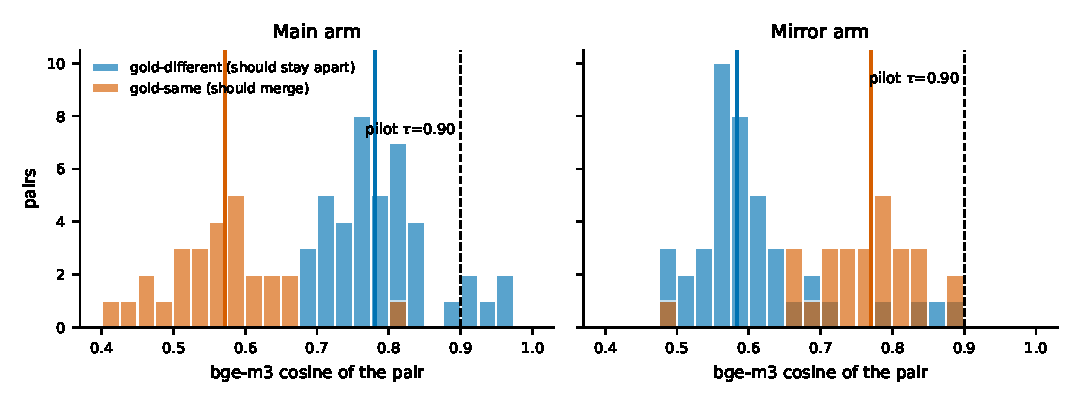
\includegraphics[width=\linewidth]{figures/d_cosine.pdf}
\caption{Raw bge-m3 cosine of the injected pair, by gold relation, per arm (Config D). Solid lines: medians. Dashed: pilot $\tau=0.90$.
All 69 pairs of each arm are drawn.}\label{fig:dcos}
\end{figure}

\paragraph{Mirror arm.} \todo{P1: Config C on the mirror arm: false merges \MirrorCoffHiFCR{} (gate off) $\to$ \MirrorClexHiFCR{} (gate on), missed merges \MirrorCoffHiMCR{} $\to$ \MirrorClexHiMCR{}. The gate helps on both arms.}

\paragraph{QA.} \todo{P1: QA accuracy \MainCoffQA{} (C off) vs \MainClexQA{} (C on); merging affects what the answerer retrieves.}

\subsection{Tier 2 v2: Hindi, Marathi and Gujarati, Configurations A--D}
\label{sec:results-v2}

The v2 arm (frozen as v2.0 before any run) has \VTwoNPairs{} injected pairs, \VTwoNDiff{} gold-different and \VTwoNSame{} gold-same
(Hindi \VTwoNHiDiff{}/\VTwoNHiSame{}, Marathi \VTwoNMrDiff{}/\VTwoNMrSame{}, Gujarati \VTwoNGuDiff{}/\VTwoNGuSame{}, as different/same),
and runs all four configurations with the 7B identity judge for A--C. It is a separate experiment from the v1.0 and mirror arms above
and is not pooled with them. Rates here are at the final memory-record level; the v2 lexicon adds Marathi and Gujarati entries that,
like the Marathi and Gujarati items, are not native-verified. These are provisional development results from one seed.

\begin{table}[t]\centering\small
% GENERATED by paper/tools/make_v2_numbers.py. Do not edit.
\begin{tabular}{llccc}
\toprule
Config & DK-Mem & FCR & MCR & QA \\
\midrule
A (English gloss) & gate off & 11/68 [0.09, 0.27] & 18/58 [0.21, 0.44] & 89/194 \\
A (English gloss) & gate on & 1/68 [0.00, 0.08] & 30/58 [0.39, 0.64] & 94/194 \\
\midrule
B (native-language fact) & gate off & 12/68 [0.10, 0.28] & 5/58 [0.04, 0.19] & 149/194 \\
B (native-language fact) & gate on & 6/68 [0.04, 0.18] & 20/58 [0.24, 0.47] & 152/194 \\
\midrule
C (verbatim) & gate off & 18/68 [0.17, 0.38] & 5/58 [0.04, 0.19] & 163/194 \\
C (verbatim) & gate on & 7/68 [0.05, 0.20] & 20/58 [0.24, 0.47] & 164/194 \\
\midrule
D (cosine, $\tau$=0.90) & gate off & 0/68 [0.00, 0.05] & 56/58 [0.88, 0.99] & 162/194 \\
D (cosine, $\tau$=0.90) & gate on & 0/68 [0.00, 0.05] & 58/58 [0.94, 1.00] & 162/194 \\
\bottomrule
\end{tabular}

\caption{Tier~2 v2 (\VTwoNPairs{} pairs; Hindi, Marathi, Gujarati), one seed, development data, provisional. FCR over the \VTwoNDiff{}
gold-different pairs, MCR over the \VTwoNSame{} gold-same pairs, 95\% Wilson intervals; QA: correct answers over all questions.}
\label{tab:results-v2}
\end{table}

\paragraph{The gate removes the kinship false merges of every LLM host.} With the gate on, false merges fall from \VTwoAOffFCR{} to
\VTwoALexFCR{} (A), \VTwoBOffFCR{} to \VTwoBLexFCR{} (B) and \VTwoCOffFCR{} to \VTwoCLexFCR{} (C). For C the change in the
gold-different merge rate is \VTwoCgateDifferentDiff{} (95\% CI \VTwoCgateDifferentDiffci{}; discordant pairs
\VTwoCgateDifferentDiscordant{}, exact McNemar $p=\VTwoCgateDifferentMcNemar$). On kinship pairs the judge alone merges
\VTwoCOffKinFCR{} gold-different pairs and none with the gate (\VTwoCLexKinFCR{}); A and B also drop to \VTwoALexKinFCR{} and
\VTwoBLexKinFCR{}. The false merges that remain are contextual-qualifier pairs (C: \VTwoCLexQualFCR{}), a class the gate does not cover.
By language, C's false merges go from \VTwoCOffHiFCR{} to \VTwoCLexHiFCR{} in Hindi, \VTwoCOffMrFCR{} to \VTwoCLexMrFCR{} in Marathi
and \VTwoCOffGuFCR{} to \VTwoCLexGuFCR{} in Gujarati; the Marathi and Gujarati cells are small and only indicative.

\paragraph{The cost is missed merges, mostly from register.} Missed merges rise from \VTwoCOffMCR{} to \VTwoCLexMCR{} for C (B:
\VTwoBOffMCR{} to \VTwoBLexMCR{}; A: \VTwoAOffMCR{} to \VTwoALexMCR{}). Most of this comes from gold-same register pairs, in which one
person is addressed with two registers: C misses \VTwoCOffRegMCR{} of them without the gate and \VTwoCLexRegMCR{} with it, because
the gate treats a register difference as evidence of two people while our labelling convention treats a shared vocative as one. In
the pre-registered kinship-only variant, in which register no longer vetoes, C keeps its false merges at \VTwoCLexKOFCR{} and misses
\VTwoCLexKOMCR{} gold-same pairs instead of \VTwoCLexMCR{}. The gold-same kinship pairs that are still blocked (\VTwoCLexKinMCR{}
for C, against \VTwoCOffKinMCR{} without the gate) are lexicon gaps rather than judge errors: one mention names the person without a
kinship term, so only one side carries the feature; a relative is described periphrastically (``mother's sister'' for
\emph{mausi}); \emph{mama ki wife} is tagged as \emph{mama} although it denotes the \emph{mami}; and a spelling variant
(\emph{naani}) is missing.

\paragraph{QA moves little.} QA accuracy is \VTwoCOffQApct\% (C, gate off) and \VTwoCLexQApct\% (gate on); B \VTwoBOffQApct\% and
\VTwoBLexQApct\%; A \VTwoAOffQApct\% and \VTwoALexQApct\%. We did not test these differences; the extra missed merges did not lower
QA accuracy on this benchmark.

\paragraph{The embedding host cannot match the judge at any threshold.} At $\tau=0.90$ Config D merges almost nothing (MCR
\VTwoDOffMCR{}). Over its full frontier (\VTwoDFrontNTaus{} distinct thresholds, none selected), the lowest false consolidation
rate D reaches at C's missed-merge rate is \VTwoDFrontCOffOff\% without the gate and, at the gated C's missed-merge rate,
\VTwoDFrontCLexLex\% with it, against C's own \VTwoCOffFCRpct\% and \VTwoCLexFCRpct\%.

% OWNER: P4 (Gujarati native), with one paragraph each from P2 (Hindi linguistics) and P3 (Marathi/lexicon): add yours as a separate
% \paragraph block at the end of this file in your own PR (append-only, so merges do not conflict). ~400 words total.
% This section is what makes the paper honest; do not shorten it to fit page limits -- cut elsewhere.
\section{Limitations and Ethics}
\label{sec:limits}

\paragraph{Scale and seeds.} One seed with greedy decoding; 36 Hindi gold-different and 27 gold-same pairs; wide intervals.
\todo{P4: state that greedy decoding makes reruns identical, so uncertainty here is over pairs, not sampling.}

\paragraph{No held-out test set.} \todo{P4: all numbers are development results; the planned independent test set (Sec.~\ref{app:repro})
is not built yet.}

\paragraph{Constructed data and conventions.} \todo{P4: templated sentences; labelling conventions; the v1 kinship city/weekday confound.}

\paragraph{Languages.} \todo{P4: results are Hindi-only; Marathi/Gujarati items exist with in-team review but were not evaluated; the
judge's behaviour in those languages is unvalidated.}

\paragraph{Lexicon.} \todo{P3: 15 Hindi entries; context-free; the reflexive \emph{apne aap} is tagged as the polite pronoun (affects 0 of
46{,}106 frozen benchmark strings); proposed Marathi/Gujarati entries are unreviewed proposals.}

\paragraph{Ethics.} \todo{P4: no personal data; constructed sentences; kinship-based assumptions; risk of encoding normative family
structures.}

\bibliographystyle{plainnat}
\bibliography{refs}
\appendix
% OWNER: P1 (lead). Appendix. Sources: DKMEM_IMPLEMENTATION.md, eval/tier2/judge_host.py, eval/tier2/judge_provenance.py,
% eval/tier2/embedder_pin.py, eval/tier2/entity_report_verified.py, tests/test_store_regression.py.
\section{Reproducibility and Evaluation Integrity}
\label{app:repro}

\paragraph{Frozen artefacts.} \todo{P1: FROZEN\_v1.0 and v1.1m benchmark files; pre-registered analysis plan pinned by sha256 before any
full-run output existed; the entity report regenerates byte-for-byte from the stored runs.}

\paragraph{A silent judge substitution.} \todo{P1: the first full run imported a judge from an external module that reused the frozen prompt
id with a different prompt and answer vocabulary; all 3105 answers were the constant string "different". Lesson: identify prompts by
content hash, not by id.}

\paragraph{Independent verification.} \todo{P1: every judge-log row is checked against the manifest's prompt id and sha256 and its raw output
is re-parsed with the strict parser; the embedder revision is checked against a registered pin; the official report entry point refuses
unverified runs. All 10 current judge logs and 28 manifests verify.}

\paragraph{Code and tests.} \todo{P1: test-suite size at submission; regression replay of the frozen Tier-1 runs through the store path.}

\end{document}
